\documentclass{article} 
\usepackage{tikz}
\usepackage{graphicx}

\begin{document} 

\begin{figure}
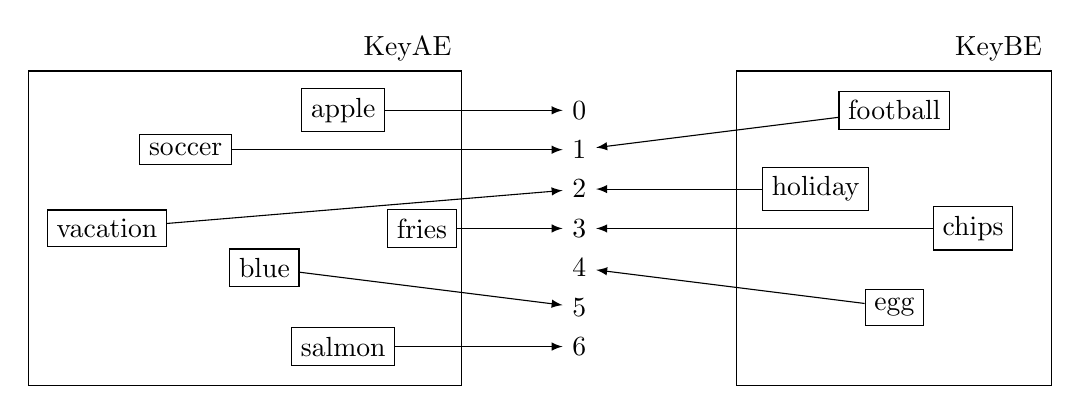
\begin{tikzpicture}
  \node[draw=black](vacation) at (-6,0) {vacation};
  \node[draw=black](fries)    at (-2,0) {fries};
  \node[draw=black](soccer)   at (-5,1) {soccer};
  \node[draw=black](apple)    at (-3,1.5) {apple};
  \node[draw=black](blue)     at (-4,-0.5) {blue};
  \node[draw=black](salmon)   at (-3,-1.5) {salmon};
  \draw (-7, -2) rectangle (-1.5, 2) node [above left] {KeyAE} ;
  
  
  \node[draw=black](holiday) at (3,0.5) {holiday};
  \node[draw=black](chips) at (5,0.0) {chips};
  \node[draw=black](football) at (4,1.5) {football};
  \node[draw=black](egg) at (4,-1) {egg};
  \draw (2, -2) rectangle (6, 2) node [above left] {KeyBE} ;
  
  \node (0) at (0,1.5) {0};
  \node (1) at (0,1.0) {1};
  \node (2) at (0,0.5) {2};
  \node (3) at (0,0.0) {3};
  \node (4) at (0,-.5) {4};
  \node (5) at (0,-1.) {5};
  \node (6) at (0,-1.5) {6};

  \draw[-latex] (vacation)--(2);
  \draw[-latex] (soccer)--(1);
  \draw[-latex] (apple)--(0);
  \draw[-latex] (fries)--(3);
  \draw[-latex] (salmon)--(6);
  \draw[-latex] (blue)--(5);
  
  
  \draw[-latex] (football)--(1);
  \draw[-latex] (chips)--(3);
  \draw[-latex] (holiday)--(2);
  \draw[-latex] (egg)--(4);

  %\draw (-0.5, -0.5) rectangle (1.5, 1.5) node [above left] {Key1} ;
\end{tikzpicture}
\caption{Mapping of individual \texttt{ModelParameter} lists to a global one.}
\end{figure}

Some text

\end{document}
